\section{Solución de Mie}

\index{Mie!solución de}\index{Esparcimiento! de luz|see{Mie}}
El problema de absorción y esparcimiento de luz por una partícula esférica de tamaño arbitrario fue resuelto por el físico alemán Gustav Mie en 1908 \cite{mie1908metallosung}. La solución de Mie consiste en expandir una onda plana monocromática, que ilumina a una esfera de tamaño y material arbitrario, en una base de armónicos esféricos vectoriales que representan una base ortogonal, cuyos elementos satisfacen las ecuaciones de Maxwell \cite{bohren1998absorption}. Al considerar las condiciones de contorno que satisfacen los campos EMs sobre la superficie de la esfera, se escriben los campos EMs dentro de la partícula y los campos esparcidos por ésta como una serie de armónicos esféricos vectoriales, cuyos coeficientes corresponden a una expansión multipolar y son conocidos como los coeficientes de Mie \cite{bohren1998absorption}. A pesar de que existen publicaciones previas a la de Mie en donde  el problema de la absorción y esparcimiento de luz es tratado de forma semejante, el trabajo de Mie destacó debido al desarrollo de relaciones recursivas que facilitan el cálculo numérico y a que discute la convergencia de los resultados \cite{horvath2009historic}. El desarrollo de una solución apta para el cálculo numérico permitió que en el artículo de Mie se describieran diez propiedades de la luz al interactuar con suspensiones diluidas de partículas esféricas \cite{mie1908metallosung}, lo que contribuyó al impacto de su solución sobre el trabajo de otros autores \cite{horvath2009historic}. El desarrollo de la solución de Mie descrito en esta sección se basa principalmente en \cite{bohren1998absorption}.

	\begin{figure}[h!]\centering
	\tdplotsetmaincoords{60}{110}
	\pgfmathsetmacro{\rvec}{1. 3}
	\pgfmathsetmacro{\thetavec}{30}
	\pgfmathsetmacro{\varphivec}{60}
\begin{tikzpicture}[scale=3.5,tdplot_main_coords]
%draw the NP
	\draw[tdplot_screen_coords,ball color=yellow, opacity = 1] (0,0,0) circle (.05);
	\draw[tdplot_screen_coords, color=yellow, opacity = 1] (0,0,0) circle (.05);


%set up some coordinates 
	\coordinate (O) at (0,0,0);

%determine a coordinate (P) using (r,\theta,\varphi) coordinates.   This command
%also determines (Pxy), (Pxz), and (Pyz): the xy-, xz-, and yz-projections
%of the point (P). 
%syntax: \tdplotsetcoord{Coordinate name without parentheses}{r}{\theta}{\varphi}
	\tdplotsetcoord{P}{\rvec}{\thetavec}{\varphivec}

%draw figure contents
%--------------------
%draw the main coordinate system axes
	\draw[thick,- latex] (0,0,0) -- (1. 5,0,0) node[anchor=north east]{$x$};
	\draw[thick,- latex] (0,0,0) -- (0,1. 5,0) node[anchor=north west]{$y$};
	\draw[thick,- latex] (0,0,0) -- (0,0,1. 5) node[anchor=south]{$z$};

%draw the main cartesian vector system 
	\draw[thick,- latex, blue] (0,0,0) -- (1,0,0) node[anchor= south east]{$\vu{e}_x$};
	\draw[thick,- latex, blue] (0,0,0) -- (0,1,0) node[anchor=north west]{$\vu{e}_y$};
	\draw[thick,- latex, blue] (0,0,0) -- (0,0,1) node[anchor= east]{$\vu{e}_z$};

%draw a vector from origin to point (P) 
	\draw[thick,color=green, - latex] (O) -- (P);
	\node at (1,. 5,1. 1) {\color{green} $\vb{r}$};

%draw projection on xy plane, and a connecting line
	\draw[dashed, color=green] (O) -- (Pxy);
	\draw[dashed, color=green] (P) -- (Pxy);
	\fill[green, opacity = .3] (O) --(Pxy)-- (P)--(O);
	\draw[- latex, tdplot_screen_coords,green](.42,.2)--(.8,.2);
	\node[tdplot_screen_coords] at (1.35,.2) {\color{green}\small Plano de esparcimiento};


%draw the angle \varphi, and label it
	%syntax: \tdplotdrawarc[coordinate frame, draw options]{center point}{r}{angle}{label options}{label}
	\tdplotdrawarc[- latex]{(O)}{0. 5}{0}{\varphivec}{anchor=south}{$\varphi$}


%set the rotated coordinate system so the x'-y' plane lies within the
	%"theta plane" of the main coordinate system
	%syntax: \tdplotsetthetaplanecoords{\varphi}
	\tdplotsetthetaplanecoords{\varphivec}

%draw theta arc and label, using rotated coordinate system
	\tdplotdrawarc[tdplot_rotated_coords, - latex]{(0,0,0)}{0. 45}{0}{\thetavec}{anchor=north}{$\theta$}

%draw some dashed arcs, demonstrating direct arc drawing
	\draw[dashed,tdplot_rotated_coords] (\rvec,0,0) arc (0:90:\rvec);
	\draw[dashed] (\rvec,0,0) arc (0:90:\rvec);

%set the rotated coordinate definition within display using a translation
%coordinate and Euler angles in the "z(\alpha)y(\beta)z(\gamma)" euler rotation convention
%syntax: \tdplotsetrotatedcoords{\alpha}{\beta}{\gamma}
	\tdplotsetrotatedcoords{\varphivec}{\thetavec}{0}

%translate the rotated coordinate system
%syntax: \tdplotsetrotatedcoordsorigin{point}
	\tdplotsetrotatedcoordsorigin{(P)}

%use the tdplot_rotated_coords style to work in the rotated, translated coordinate frame
	\draw[thick,tdplot_rotated_coords,- latex, purple] (0,0,0) -- (. 3,0,0) node[anchor=north west]{{\color{black}$\vu{e}_\theta,$}$\vu{e}_{\parallel}^s$};
	\draw[thick,tdplot_rotated_coords,- latex,black] (0,0,0) -- (0,. 3,0) node[anchor=west]{$\vu{e}_\varphi$};
	\draw[thick,tdplot_rotated_coords,- latex,purple] (0,0,0) -- (0,-. 3,0) node[anchor= north west]{$\vu{e}_{\perp}^s$};
	\draw[thick,tdplot_rotated_coords,- latex] (0,0,0) -- (0,0,. 3) node[anchor=south]{$\vu{e}_r$ };



%set the rotated coordinate definition within display using a translation
%coordinate and Euler angles in the "z(\alpha)y(\beta)z(\gamma)" euler rotation convention
%syntax: \tdplotsetrotatedcoords{\alpha}{\beta}{\gamma}
	\tdplotsetrotatedcoords{\varphivec}{0}{0}

%translate the rotated coordinate system
%syntax: \tdplotsetrotatedcoordsorigin{point}
	\tdplotsetrotatedcoordsorigin{(Pxy)}

	\draw[thick,tdplot_rotated_coords,- latex, purple] (0,0,0) -- (. 3,0,0) node[anchor= west]{$\vu{e}_{\parallel}^i$};
	\draw[thick,tdplot_rotated_coords,- latex, blue] (0,0,0) -- (0,0,. 3) node[anchor= west]{$\vu{e}_z$};	
	\draw[thick,tdplot_rotated_coords,- latex, purple] (0,0,0) -- (0,-. 3,0) node[anchor= north west]{$\vu{e}_{\perp}^i$};



% Plane Wave
	\foreach \i in {-7,...,-2}{
		\draw[thick,tdplot_screen_coords,red, - latex] (\i/10,0,0)--(\i/10,1,0);}
	\node[tdplot_screen_coords] at (-4.5/10,1.1,0){\color{red}$\vb{k}_i$};
	\node[tdplot_screen_coords] at (-4.5/10,-.1,0){\small \color{red}Haz incidente};
\end{tikzpicture}
%
\caption{Diagrama del plano de esparcimiento (en verde) definido por el vector $\vb{r}$, posición donde se evalúan los campos EMs, y el vector $\vu{e}_z$, cuando una onda plana monocromática propagándose en dirección $z$ (en rojo) ilumina a una partícula arbitraria.  La base cartesiana para vectores se muestra en azul, mientras que la base esférica se muestra en negro.  Las direcciones paralelas $\parallel$ y perpendiculares $\perp$ al plano de incidencia  para el campo eléctro incidente, denotado por el subíndice $i$ y el esparcido, denotado por el subíndice $s$, se muestran en morado; el haz incidente se muestra en rojo.}\label{fig:PlanoEsparcimiento}
	\end{figure}	

Para  el estudio del esparcimiento por una partícula arbitraria inmersa en un medio con índice de refracción $n_m$, denominado  matriz, se considera que la partícula es iluminada por una onda plana monocromática con una longitud de onda $\lambda$, cuya dirección de propagación define la dirección $z$, es decir,
	\begin{align}
	\vb{E}^i = (E_x^i \vu{e}_x + E_y^i \vu{e}_y)e^{i(k z - \omega t)},
	\label{eq:Exyi}
	\end{align}
donde $k = 2\pi n_m /\lambda$ es el número de onda. En la Fig.  \ref{fig:PlanoEsparcimiento} se muestra  una partícula localizada en el origen,  iluminada por una onda plana monocromática [Ec. \eqref{eq:Exyi}] que se propaga en la dirección $z$. De forma análoga al plano de incidencia, se construye el plano de esparcimiento (en verde en la Fig. \ref{fig:PlanoEsparcimiento}), con el vector de dirección del esparcimiento $\vu{e}_r$ y la dirección del haz incidente $\vu{e}_z$, que define las componentes ortogonales $\perp$ y paralelas $\parallel$ de los campos EMs, así como su polarización. \index{Plano!de esparcimiento} \index{Polarización!respecto al plano de esparcimiento} Los vectores unitarios perpendicular y paralelo al plano de esparcimiento de la onda incidente, $\vu{e}_{\perp}^i$  y $\vu{e}_{\parallel}^i$, respectivamente, y de los campos EMs esparcidos $\vu{e}_{\perp}^s$ y $\vu{e}_{\parallel}^s$ están dados por%
\begin{subequations} \index{Polarización!respecto al plano de esparcimiento!paralela ($\parallel$)}\index{Polarización!respecto al plano de esparcimiento!perpendicular ($\perp$)}\vspace*{-1em}

	\eqhalf{\vu{e}_{\perp}^i =-\, \hat{e}_\varphi  = \sin\varphi\,\vu{e}_x - \cos\varphi\,\vu{e}_y,}	
	\eqhalf{\vu{e}_{\parallel}^i = \cos\varphi\,\vu{e}_x + \sin\varphi\,\vu{e}_y,}	
	\label{eqs:vecInc}\end{subequations}	\begin{subequations}
	\eqhalf{\vu{e}_{\perp}^s= - \, \vu{e}_\varphi,}	
	\eqhalf{\vu{e}_{\parallel}^s = \vu{e}_\theta.}	
	\label{eqs:vecScat}\end{subequations}\vspace*{-1em}

\noindent Al despejar $\vu{e}_x$ y $\vu{e}_y$  de las Ecs. \eqref{eqs:vecInc} y reescribirlos en la base de los vectores unitarios en la dirección perpendicular y normal al plano de esparcimiento como $\vu{e}_x = \sin\varphi\,\vu{e}_{\perp}^i + \cos\varphi\,\vu{e}_{\parallel}^i, $ y $\vu{e}_y = - \cos\varphi \,\vu{e}_{\perp}^i + \sin\varphi\,\vu{e}_{\parallel}^i$, se obtiene que el campo eléctrico incidente $\vb{E}^i$ [Ec. \eqref{eq:Exyi}] se puede escribir como
\begin{align}
\vb{E}^i = [(\cos\varphi E_{x}^i + \sin\varphi E_{y}^i)\vu{e}_{\perp}^i +
			 (\sin\varphi E_{x}^i - \cos\varphi E_{y}^i)\vu{e}_{\parallel}^i]
			 e^{ikz}
			 = E_{\perp}^i  \vu{e}_{\perp}^i + E_{\parallel}^i\vu{e}_{\parallel}^i,
		\label{eq:EIncidente}
\end{align}
en donde se omite el término de la fase temporal $e^{-i\omega t}$ y la fase espacial $e^{ikz}$ se incluye en los coficientes $E_\perp^i$ y $E_\parallel^i$. Adicionalmente, al considerar para el campo eléctrico esparcido  únicamente los términos que corresponden al campo lejano, es decir, el término con componentes transversales, que decae como $r^{-1}$ y cumple con la relación $kr\ll 1$, el campo esparcido $\vb{E}^s$ puede escribirse como \cite{bohren1998absorption}\index{Electromagnéticos!campos!lejano} \vspace*{-1em}
	\begin{align}
	\vb{E}^s \propto \frac{e^{ikr}}{-ikr}\vb{E_0}^s 
			=  \frac{e^{ikr}}{-ikr}
			\qty( E_{\perp}^s  \vu{e}_{\perp}^s + E_{\parallel}^s \vu{e}_{\parallel}^s), \label{eq:ELejano}
	\end{align}
en donde  $\vb{E_0}^s$ es la amplitud del campo esparcido,  $ E_{\perp}^s$ y  $ E_{\parallel}^s$ sus componentes en la base de los vectores paralelo y perpendicular al plano de esparcimiento [Ec. \eqref{eqs:vecScat}]. Asimismo, es posible relacionar al campo eléctrico esparcido $\vb{E}^s$ por una partícula localizada en el centro de coordenadas  [Ec. \eqref{eq:ELejano}] con el  campo eléctrico incidente $\vb{E}^i$ [Ec. \eqref{eq:EIncidente}],  mediante el operador de esparcimiento de campo lejano  $\mathbb{F}(\vu{k}^i,\vu{k}^s)$ \index{Electromagnéticos!campos!diadica de campo lejano} \cite{tsang2000scattering}
	\begin{align}
	\vb{E}^s = \frac{e^{i\vb{k}^s\cdot\vb{r}}}{r}\mathbb{F}(\vu{k}^i,\vu{k}^s)\vb{E}^i,
	\label{eq:FarFieldDyadic}
	\end{align}
donde $\mathbb{F}$ depende de la dirección de la onda plana incidente $\vu{k}^i$ y de la dirección del campo eléctrico esparcido $\vu{k}^s$. Al considerar la forma asintótica del campo eléctrico esparcido [Ec. \eqref{eq:ELejano}] y su relación con el campo eléctrico incidente [Ec. \eqref{eq:FarFieldDyadic}], se pueden relacionar las componentes perpendiculares del campo esparcido y el campo incidente de una onda plana en la base de los vectores perpendiculares y paralelos al plano de incidencia mediante la matriz de esparcimiento $\mathbb{S}$ \index{Esparcimiento!matriz de} \cite{bohren1998absorption} \vspace*{-1em}
	\begin{align}
	\mqty(E_{\parallel}^s\\E_{\perp}^s) = 
		\frac{e^{ik(r-z)}}{-ikr} \mqty(S_2&S_3\\S_4&S_1)
	\mqty(E_{\parallel}^i\\E_{\perp}^i),\label{eq:MEsparcimientoGral}
	\end{align}
en donde $S_j = S_j(\theta,\varphi)$, con $j=1,2,3$ y $4$, son funciones complejas, además de que las componentes de la matriz de esparcimiento en la Ec. \eqref{eq:MEsparcimientoGral} dependen en general de la geometría de la partícula iluminada por la onda plana.

	\subsection{Solución a la ecuación de onda con simetría esférica}


Las ecuaciones de Maxwell, al considerar una región del espacio sin fuentes y campos EMs armónicos en el tiempo, se reescriben como \cite{jackson1999electrodynamics} \index{Maxwell!ecuaciones de!transformada de Fourier de las}

	\begin{subequations}
	\eqhalf{\nabla\cdot \vb{E} = 0, }
	\eqhalf{\nabla\cdot \vb{H} = 0,}
	\eqhalf{\nabla \times \vb{E} = i\omega\mu \vb{H}, \label{seq:FLArm}}
	\eqhalf{\nabla\times\vb{H} = - i \omega\varepsilon(\omega) \vb{E}, }	
	\label{eqs:MaxwellArm}
	\end{subequations} \vspace*{-1em}
	
\noindent	
en donde $\vb{H} = \vb{B}/\mu$ es el campo H, y la función dieléctrica $\varepsilon(\omega)$ y la permeabilidad magnética $\mu$ del material son funciones continuas. Al desacoplar las ecuaciones de Maxwell, se concluye que los campos EMs son soluciones a la ecuación de Helmholz vectorial\cite{jackson1999electrodynamics}\index{Ecuación!de Helmholtz}

	\begin{subequations}
	\eqhalf{\nabla^2 \vb{E}- k^2 \vb{E} = \vb{0},}
	\eqhalf{\nabla^2 \vb{H}- k^2 \vb{H} = \vb{0},}
	\label{eq:Helmholtz}
	\end{subequations} \vspace*{-1em}

\noindent	
en donde $k = n k_0$ es la magnitud del vector de onda, $n$ es el índice de refracción en la región del espacio donde se evalúan los campos EMs [Ec. \eqref{eq:indice}] y $k_0 = \omega / c$ es la relación de dispersión en el vacío [Ec. \eqref{eq:dispersion}].

Se propone un campo vectorial $\vb{M}$ tal que \cite{bohren1998absorption}
	\begin{align}
	\vb{M} &= \nabla \times \left(\vb{r} \psi\right),
	\label{eq:MrotCPsi}
	\end{align}
donde $\psi$ es una función escalar y $\vb{r}$ el vector de posición; dado que $\vb{M}$ es el rotacional de  $\vb{r}\psi$, se cumple que $\nabla\cdot \vb{M} = \vb{0}$, y que $\vb{M}$ y $\vb{r}$ son vectores perpendiculares\footnote{Empleando la convención de la suma de Einstein y con $\epsilon_{ijk}$ el símbolo de  Levi-Civita: \mbox{$M_i = [\nabla\times(\vb{r}\psi)]_i =  \epsilon_{ijk}\partial_j(r_k\psi) =\psi\epsilon_{ijk}\partial_j(r_k) -\epsilon_{ikj}r_k\partial_j\psi  =\psi[\nabla\times\vb{r}]_i - [\vb{r}\times\nabla\psi]_i = - [\vb{r}\times\nabla\psi]_i$}.}. La  ecuación de Helmholtz para $\vb{M}$, dado que el operador laplaciano y el rotacional conmutan\footnote{ Para un campo vectorial arbitrario $\vb{A}$ se cumple que $\nabla^2\vb{A} = \nabla(\nabla\cdot\vb{A}) - \nabla\times(\nabla\times\vb{A})$, por lo que el rotacional del laplaciano de $\vb{A}$ es $ \nabla\times( \nabla^2\vb{A})=\nabla\times[\nabla(\nabla\cdot\vb{A})  ]-  \nabla\times[\nabla\times(\nabla\times \vb{A})] = -  \nabla\times[\nabla\times(\nabla\times \vb{A})] $ pues el rotacional del gradiente de cualquier función es nulo. Además, al sustituir $\vb{A}\to \nabla\times\vb{A}$ en la expresión del laplaciano de $\vb{A}$ y  considerando que la divergencia del rotacional de cualquier función es nulo, se obtiene que$ \nabla^2(\nabla\times\vb{A})=\nabla[\nabla\cdot(\nabla\times\vb{A})  ]-  \nabla\times[\nabla\times(\nabla\times \vb{A})] = -  \nabla\times[\nabla\times(\nabla\times \vb{A})] $. Por tanto, $\nabla^2$ y $\nabla\times$ son operadores que conmutan.}, es
	\begin{align*}
	\nabla^2 \vb{M} + k^2 \vb{M} = \nabla\times \left[ \nabla^2\left(\vb{r} \psi\right)  
											+ k^2  \left(\vb{r} \psi\right) \right],
	\end{align*}
y como se cumple que\footnote{$[\nabla^2 (\vb{r}\psi)]_i = \partial^2_{jj}(r_i\psi)= \partial_j [\partial_j(r_i)\psi+r_i\partial_j\psi] =\partial_{jj}{r_i} + 2 \partial_jr_i\partial_j\psi+r_i\partial^2_{jj}\psi$, donde $\partial_j r_i = \delta_{ij}$ con $\delta_{ij}$ la delta de Kronecker,\index{Kronecker!delta de} por lo que se cumple que $[\nabla^2 (\vb{r}\psi)]_i = 2\partial_i\psi+r_i\partial_{jj}\psi = 2[\nabla\psi]_i + [\vb{r}\nabla^2\psi]_i$.}  $\nabla^2 (\vb{r}\psi)=2\nabla\psi+\vb{r}\nabla^2\psi$ y que $\nabla\times(\nabla \psi)=0$, la ecuación de Helmholtz para $\vb{M}$ puede reescribirse como
	\begin{align}
	\nabla^2 \vb{M} + k^2\vb{M}  = \nabla\times\left[\vb{r}\left( \nabla^2\psi+k^2\psi \right) \right].
	\end{align}
Adicional a $\vb{M}$, se define el vector $\vb{N}$ como \cite{bohren1998absorption} 
	\begin{align}
	\vb{N} = \frac{\nabla\times \vb{M}}{k}, \label{eq:NrotM/k}
	\end{align}
cuyo laplaciano es $\nabla^2 \vb{N} = \nabla^2( \nabla\times \vb{M} /k) =  \nabla\times (\nabla^2\vb{M} /k) $, y por tanto la ecuación de Helmholtz para $\vb{N}$ es
%	
	\begin{align*}
	\nabla^2 \vb{N} + k^2 \vb{N} =  \nabla\times \left( \frac{\nabla^2 \vb{M}}{k} \right) + k \nabla\times \vb{M} 
		 = \frac{1}{k} \nabla\times \left( \nabla^2 \vb{M} + k^2  \vb{M} \right).
	\end{align*}\noindent
%
Los campos $\vb{M}$ y $\vb{N}$ cumplen con la  ecuación de Helmholtz vectorial [Ec. \eqref{eq:Helmholtz}] si, y sólo si, la función escalar $\psi$ cumple con la ecuación de Helmholtz escalar $\nabla^2 \psi + k^2 \psi = 0$. Si este es el caso, entonces, el rotacional de $\vb{N}$ está dado por
	\begin{align}
	\nabla\times \vb{N} &= \nabla\times \qty(\frac{\nabla\times \vb{M}}{k})  
						= \frac{\nabla\qty(\nabla\cdot\vb{M})-\nabla^2\vb{M}}{k}
						= - \frac{\nabla^2 \vb{M}}{k}
						= \frac{k^2 \vb{M}}{k}
						= k \vb{M}.\label{eq:rotN}
	\end{align}\noindent
%
Los campos vectoriales $\vb{M}$ y $\vb{N}$ son conocidos como los \emph{armónicos esféricos vectoriales}\index{Armónicos esféricos vectoriales}, $\psi$ como su función generadora y $\vb{r}$ como el vector de guía o vector piloto \cite{bohren1998absorption}. Los armónicos esféricos vectoriales $\vb{M}$ y $\vb{N}$  cumplen con tener divergencia nula y que el rotacional de uno es proporcional al otro [Ecs. \eqref{eq:NrotM/k} y \eqref{eq:rotN}], es decir, que cumplen con las ecuaciones de Maxwell [Ecs. \eqref{eqs:MaxwellArm}] siempre que se cumpla que\index{Armónicos esféricos vectoriales!función generadora de los}\vspace*{-.75em}
	\begin{tcolorbox}[title = $\mathbf{\psi}$: Función generadora de los armónicos esféricos vectoriales, ams align ]
	\nabla^2 \psi + k^2 \psi  = 0.\label{eq:AV_psi}
	\end{tcolorbox}

Cuando se considera una partícula esférica de radio $a$ e índice de refracción $n_p$, inmersa en un medio denominado matriz con índice de refracción $n_m$ (ver Fig. \ref{fig:EsferaA}), iluminada por una onda plana monocromática propagándose a lo largo del eje $z$, es conveniente emplear coordenadas esféricas $(r, \theta, \varphi)$, en las que la función generadora de los armónicos esféricos vectoriales debe cumplir con la ecuación \index{Armónicos esféricos vectoriales!función generadora de los}
	\begin{align}
	\frac{1}{r^2} \pdv{r}\qty(r^2\pdv{\psi}{r})+ 
	\frac{1}{r^2\sin\theta}\pdv{\theta}\qty(\sin\theta\pdv{\psi}{\theta})
	 + \frac{1}{r^2\sin^2\theta}\pdv[2]{\psi}{\varphi} + k^2 \psi =0. \label{eq:AEV_psi}
	\end{align}
Al resolver la Ec. \eqref{eq:AEV_psi} es posible construir un conjunto de funciones linealmente independientes que sean una base para los campos EMs incidente, esparcido y dentro de la esfera, lo que permite determinar, mediante las condiciones a la frontera de los campos EMs, la forma de la matriz de esparcimiento [Ec. \eqref{eq:MEsparcimientoGral}].

	\begin{figure}[h!]\centering
	%set the plot display orientation
	%synatax: \tdplotsetdisplay{\theta_d}{\varphi_d}
		\tdplotsetmaincoords{60}{110}
	%define polar coordinates for some vector
	%TODO: look into using 3d spherical coordinate system
		\pgfmathsetmacro{\rvec}{1. 3}
		\pgfmathsetmacro{\thetavec}{30}
		\pgfmathsetmacro{\varphivec}{60}	
\begin{tikzpicture}[scale=4,tdplot_main_coords]

%set up some coordinates 
	\coordinate (O) at (0,0,0);

%determine a coordinate (P) using (r,\theta,\varphi) coordinates.   This command
%also determines (Pxy), (Pxz), and (Pyz): the xy-, xz-, and yz-projections
%of the point (P). 
%syntax: \tdplotsetcoord{Coordinate name without parentheses}{r}{\theta}{\varphi}
	\tdplotsetcoord{P}{\rvec}{\thetavec}{\varphivec}

%draw figure contents
%--------------------

%Draw the NP
	\draw[tdplot_screen_coords,ball color=yellow, opacity = 1] (O) circle (. 25);
	\draw[tdplot_screen_coords, color=yellow, opacity = 1] (O) circle (. 25);
	\draw[color=blue, -, thick] (0,0,0) -- (. 18,-. 18,. 18);	
	\node at (. 09,-. 09,. 15){\color{blue} $a$};
	\node at (. 25,-. 25,-. 05){$n_m$};
	\node at (. 01,-. 18,-. 1){$n_p$};		
	
%draw the main coordinate system axes
	\draw[thick,- latex] (0,0,0) -- (. 8,0,0) node[anchor=north east]{$x$};
	\draw[thick,- latex] (0,0,0) -- (0,. 8,0) node[anchor=north west]{$y$};
	\draw[thick,- latex] (0,0,0) -- (0,0,. 8) node[anchor=south]{$z$};

%draw a vector from origin to point (P) 
	\draw[thick,color=green, - latex] (O) -- (P);
	\node at (1,. 6,1. 2) {\color{green} $\vb{r}$};
	
%draw projection on xy plane, and a connecting line
	\draw[dashed, color=green] (O) -- (Pxy);
	\draw[dashed, color=green] (P) -- (Pxy);
%	\fill[green, opacity = . 3] (O) --(Pxy)-- (P)--(O);	

%draw the angle \varphi, and label it
	%syntax: \tdplotdrawarc[coordinate frame, draw options]{center point}{r}{angle}{label options}{label}
	\tdplotdrawarc[- latex]{(O)}{0. 6}{0}{\varphivec}{anchor=north}{$\varphi$}


%set the rotated coordinate system so the x'-y' plane lies within the
	%"theta plane" of the main coordinate system
	%syntax: \tdplotsetthetaplanecoords{\varphi}
	\tdplotsetthetaplanecoords{\varphivec}

%draw theta arc and label, using rotated coordinate system
	\tdplotdrawarc[tdplot_rotated_coords, - latex]{(0,0,0)}{0. 6}{0}{\thetavec}{anchor=north east}{$\theta$}

% Plane Wave
	\foreach \i in {-3,...,3}{
		\draw[thick,tdplot_screen_coords,red, - latex] (-.8+\i/10,-.3,0)--(-.8+\i/10,.7,0);}
	\node[tdplot_screen_coords] at (-8/10,+.8,0){\color{red}$\vb{k}_i$};
	\node[tdplot_screen_coords] at (-8/10,-.4,0){\small \color{red}Haz incidente};
\end{tikzpicture}	
		\caption{ Esfera de radio $a$ e ínidce de refracción $n_p$, inmersa en una matriz con índice $n_m$. La esfera es iluminada por una onda plana monocromática con vector de onda $\vb{k}_i$, que se propaga en la dirección $\hat{e}_z$.}\label{fig:EsferaA}
	\end{figure}	
	
Para resolver la Ec. \eqref{eq:AEV_psi} se emplea el método de separación de variables, proponiendo como solución $\psi= R(r)\Theta(\theta) \Phi(\varphi)$. Para que $\psi$ sea solución a la Ec.  \eqref{eq:AEV_psi}, las funciones $R(r),\, \Theta(\theta), \mbox{ y } \Phi(\varphi)$ deben cumplir las siguientes ecuaciones
	\begin{align}
	\frac{1}{\Phi}\dv[2]{\psi}{\varphi} &+ m^2 \Phi =0, \label{eq:Phi}\\
	\frac{1}{\sin\theta}\dv{\theta}\qty(\sin\theta\dv{\Theta}{\theta}) &+ 	\qty[\ell(\ell+1)- \frac{m^2}{\sin^2\theta}]\Theta =0,\label{eq:Theta}\\
	\dv{r}\qty(r^2\dv{R}{r}) &+ \qty[ k^2 r^2 - \ell (\ell +1)] R =0, 	\label{eq:Req}
	\end{align}
en donde tanto $\ell$  como $m$ son constantes que se determinan mediante las condiciones impuestas a $\psi$. Dado que $\psi$ debe ser una función con periodicidad $2\pi$ en $\varphi$, es decir que $\psi(\varphi) = \psi(\varphi+2\pi)$, las soluciones linealmente independientes de la Ec. \eqref{eq:Phi} son \index{Armónicos esféricos vectoriales!función generadora!solución azimutal de la}

	\begin{subequations}
	\eqhalf{\Phi_e(\varphi) = \cos(m\varphi),}
	\eqhalf{\Phi_o(\varphi) = \sin(m\varphi),}
	\label{eq:SinCos} 
	\end{subequations} \vspace{-1em}
	
\noindent con $m$ un número natural (incluido el cero) y donde los subíndices $e$ y $o$ hacen referencia a que son funciones pares (\emph{even}, $e$) e impares (\emph{odd}, $o$), respectivamente. Las funciones $\sin(m\varphi)$ y $\cos(m\varphi)$ obedecen las siguientes relaciones de ortogonalidad
 	\begin{subequations}
	\begin{align}
	\int_0^{2\pi} \sin(m\varphi) &\cos(m' \varphi) \dd\varphi = 0 \qquad \forall\, m,m',\label{seq:ortSinCos}\\
	\int_0^{2\pi} \sin(m\varphi) \sin(m'\varphi)\dd\varphi &=  \int_0^{2\pi} \cos(m\varphi) \cos(m'\varphi)\dd\varphi  = \delta_{m,m'}\frac{\pi}{2},\label{seq:ortCos2}
	\end{align}\label{eq:ortSinCos}
 	\end{subequations}
en donde $\delta_{m,m'}$ es la delta de Kronecker.\index{Kronecker!delta de}\index{Ortogonalidad!seno y coseno, relaciones de}

Al realizar el cambio de variable $\mu = \cos\theta$ en la Ec. \eqref{eq:Theta}, ésta se reescribe como
	\begin{align*}
	\qty(1-\mu^2) \dv[2]{\Theta}{\mu} - 2 \mu \dv{\Theta}{\mu} + \qty[\ell(\ell+1)-\frac{m^2}{(1-\mu^2)}]\Theta= 0,
	\end{align*}\index{Armónicos esféricos vectoriales!función generadora!solución polar de la}\index{Ecuación!asociada de Legendre}\index{Legendre!ecuación asociada de}
\hspace{-.5em}cuyas soluciones son	las \emph{funciones asociadas de Legendre} $P_\ell^m(\cos\theta)$ de grado $\ell$ y orden $m$  \cite{arfken2001methods}, imponiendo que $\ell = m, m+1,m+2,\ldots$ para  que la Ec. \eqref{eq:Theta} sea finita en $\theta = 0$ y $\theta = \pi$. Las funciones asociadas de Legendre cumplen con la relación de ortogonalidad 
	\begin{align}
	\int_{-1}^1P_\ell^m(\mu) P_{\ell'}^md\mu = \delta_{\ell,\ell'}\frac{2}{2\ell+1}\frac{(\ell+m)!}{(\ell-m)!}.
	\label{eq:ortLegendre}
	\end{align}\index{Legendre!polinomios de}\index{Legendre!funciones asociadas de}\index{Ortogonalidad!funciones asociadas de Legrende, relaciones de}\index{Legendre!funciones asociadas de!relaciones de ortogonalidad de las}
\hspace{-.5em}Asimismo, las funciones asociadas de Legendre se reducen a los polinomios de Legendre cuando $m=0$, además de que las funciones asociadas y los polinomios de Legendre se relacionan mediante la siguiente identidad  \cite{arfken2001methods}
	\begin{align}
	P_\ell^m (\mu) = (1-\mu^2)^{m/2}\dv[m]{P_\ell(\mu)}{\mu},
	\label{eq:Legendre}
	\end{align}
de donde se deduce  que $P_\ell^m(\pm 1)=0$ para toda $m$ distinta de cero.

Para resolver la Ec. \eqref{eq:Req} se emplea el cambio de variable $\rho = k r$ y se define la función $Z =R\sqrt{\rho}$, por lo que la ecuación radial se reescribe como \index{Armónicos esféricos vectoriales!función generadora!solución radial de la}\index{Ecuación!esférica de Bessel}\index{Bessel!ecuación esférica de}
	\begin{align}
	\rho \dv{\rho}\qty(\rho\dv{Z}{\rho})+\qty[\rho^2-\qty(\ell+\frac12)^2] Z = 0,
	\label{eq:rho}
	\end{align}
cuyas soluciones son las \emph{funciones esféricas de Bessel} $j_\ell$ y $y_\ell$, o cualquier combinación lineal de ellas, por lo que de forma general las soluciones de la Ec. \eqref{eq:rho} son \cite{arfken2001methods} \index{Bessel!funciones esféricas de}

	\begin{subequations}
	\eqhalf{j_\ell (\rho) = \sqrt{\frac{\pi}{2\rho}} J_{\ell+1/2}(\rho), \label{eqs:jn}}
	\eqhalf{y_\ell (\rho) = \sqrt{\frac{\pi}{2\rho}} Y_{\ell+1/2}(\rho), \label{eqs:yn}}
	\eqhalf{h_\ell^{(1)} (\rho) = j_\ell(\rho) + i y_\ell(\rho), \label{eqs:h1}}
	\eqhalf{h_\ell^{(2)} (\rho) =  j_\ell(\rho) - i y_\ell(\rho), \label{eqs:h2}}
	\label{eq:SphBessel}
	\end{subequations}

\noindent	
en donde $J_\ell$ y $Y_\ell$ son las \emph{funciones de Bessel del primer y segundo tipo}, respectivamente, y $h_\ell$ son las \emph{funciones esféricas de Bessel del tercer tipo}, también denominadas como \emph{funciones esféricas de Hankel}. Todas las funciones esféricas de Bessel $z_\ell$ ---donde $z_\ell$ es cualquier función de las Ecs. \eqref{eq:SphBessel}--- pueden ser calculadas mediante relaciones de recurrencia\footnote{Todas las funciones esféricas de Bessel cumplen \cite{arfken2001methods}: $	z_{\ell-1}(\rho) + z_{\ell+1}(\rho) =(2\ell+1)z_\ell(\rho)/\rho$ y $(2\ell + 1) \dv*{z_\ell(\rho)}{\rho} = \ell z_{\ell-1}(\rho) - (\ell+1)z_{\ell+1}(\rho)$, con  $j_0(\rho) = \sin\rho / \rho$ y $j_1(\rho) = \sin\rho / \rho^2- \cos\rho/\rho$, $y_0(\rho) = -\cos\rho/\rho$ y $y_1(\rho) = -\cos\rho/\rho^2-\sin\rho/\rho$.\index{Bessel!funciones esféricas de!relaciones de recurrencia de las}}  \cite{arfken2001methods}\index{Hankel!funciones esféricas de}\index{Hankel|see{Bessel}}.

Dado que las soluciones para la ecuación azimutal son las Ecs. \eqref{eq:SinCos}, para la polar, Ec. \eqref{eq:Legendre} y para la radial, Ecs. \eqref{eq:SphBessel}, las funciones generadoras de los armónicos esféricos vectoriales son\index{Armónicos esféricos vectoriales!función generadora!solución general}\begin{subequations}\vspace*{-2em}

	\eqhalf{\psi_{em\ell} = \cos(m\varphi) P_\ell^m( \cos \theta) z_\ell(k r),}
	\eqhalf{\psi_{om\ell} = \sin(m\varphi) P_\ell^m( \cos \theta) z_\ell(k r).}
	\label{eq:psieo}	\end{subequations}\vspace*{-.5em}

\noindent Al emplear las Ecs. \eqref{eq:psieo} en la Ec. \eqref{eq:MrotCPsi} se obtiene como resultado $\vb{M}_{em\ell}$ y $\vb{M}_{om\ell}$, dados por las expresiones \vspace{-.5em}
	\begin{subequations}
	\begin{tcolorbox}[title = Armónicos esféricos vectoriales $\vb{M}_{em\ell}$ y $\vb{M}_{om\ell}$, ams align ]
	\vb{M}_{em\ell} = &-m\sin(m\varphi)z_\ell(kr) \frac{P_\ell^m(\cos\theta)}{\sin\theta}\,\vu{e}_\theta
					-\cos(m\theta)z_\ell(kr) \dv{P_\ell^m(\cos\theta)}{\theta}(\cos\theta)\,\vu{e}_\varphi,\label{seq:Meml} \\
	\vb{M}_{om\ell} = & m\cos(m\varphi)z_\ell(kr) \frac{P_\ell^m(\cos\theta)}{\sin\theta}\,\vu{e}_\theta
					-\sin(m\theta)z_\ell(kr) \dv{P_\ell^m(\cos\theta)}{\theta}(\cos\theta)\,\vu{e}_\varphi.	\label{seq:Moml}				
	\end{tcolorbox}\vspace*{-.75em} \noindent
%
Para el cálculo de $\vb{N}_{em\ell}$ y $\vb{N}_{om\ell}$ se sustituyen las Ecs. \eqref{seq:Meml} y \eqref{seq:Moml} en la Ec. \eqref{eq:NrotM/k}. Para simplificar las expresiones de las componentes radiales de  $\vb{N}_{em\ell}$ y $\vb{N}_{om\ell}$, se agrupan los términos que dependen de $\varphi$ y $kr$ y, dado que las funciones asociadas de Legendre cumplen con la relación 
\begin{align*}
-\ell(\ell+1) P_\ell^m (\cos\theta)= \frac{1}{\sin\theta}\dv{\theta}\qty(\sin\theta\dv{P_\ell^m(\cos\theta)}{\theta}) - \frac{m^2}{\sin^2\theta}P_\ell^m(\cos\theta),
\end{align*}
que es una consecuencia de la Ec. \eqref{eq:Theta}, las expresiones de $\vb{N}_{em\ell}$ y $\vb{N}_{om\ell}$ son \index{Armónicos esféricos vectoriales!$\vb{M}$ y $\vb{N}$} \vspace*{-.75em}
%
	\begin{tcolorbox}[title = Armónicos esféricos vectoriales $\vb{N}_{em\ell}$ y $\vb{N}_{om\ell}$, ams align, breakable ]
	\vb{N}_{em\ell} =&\cos(m\varphi) \frac{z_\ell(kr)}{kr} \ell(\ell+1)P_\ell^m(\cos\theta)\,\vu{e}_r\notag\\
	&+ \cos(m\varphi)  \frac{1}{kr} \dv{(kr)}\qty\Big[kr\, z_\ell(kr)] \dv{P_\ell^m(\cos\theta)}{\theta}(\cos\theta)\,\vu{e}_\theta
	 \label{seq:Neml} \\
		&- m \sin(m\varphi) \frac{1}{kr} \dv{(kr)}\qty\Big[kr\, z_\ell(kr)] \frac{P_\ell^m(\cos\theta)}{\sin\theta}
		 \,\vu{e}_\varphi, \notag\\			
	\vb{N}_{om\ell} =&\sin(m\varphi)\frac{z_\ell(kr)}{kr} \ell(\ell+1)P_\ell^m(\cos\theta)\,\vu{e}_r \notag\\
	&+ \sin(m\varphi)  \frac{1}{kr} \dv{(kr)}\qty\Big[kr\, z_\ell(kr)] \dv{P_\ell^m(\cos\theta)}{\theta}(\cos\theta) \,\vu{e}_\theta
	 \label{seq:Noml} \\
		&+ m \cos(m\varphi) \frac{1}{kr} \dv{(kr)}\qty\Big[kr\, z_\ell(kr)] \frac{P_\ell^m(\cos\theta)}{\sin\theta}
		\, \vu{e}_\varphi. \notag							
	\end{tcolorbox}\label{eq:AEV}
	\end{subequations}\vspace*{-.75em} \noindent
%
Los armónicos esféricos vectoriales son solución a la ecuación de Helmholtz, por lo que cualquier solución de los campos EMs puede escribirse como una serie infinta en términos de las Ecs. \eqref{eq:AEV}. 

Para resolver el problema de los campos EMs esparcidos por una partícula esférica, esto es, determinar las componentes de la matriz de esparcimiento $\mathbb{S}$ de la Ec. \eqref{eq:MEsparcimientoGral}, se expande una onda plana monocromática $\vb{E}^i$ en la base de los armónicos esféricos vectoriales, haciendo uso de sus condiciones de ortogonalidad, calculadas a partir de la relaciones de ortogonalidad de las Ecs. \eqref{eq:ortSinCos} y \eqref{eq:ortLegendre}, dando como resultado que los armónicos esféricos vectoriales son ortogonales cuando tienen paridad distinta y cuando se realiza el producto interior entre $\vb{M}$ y $\vb{N}$, es decir \index{Armónicos esféricos vectoriales!relaciones de ortogonalidad de los}\index{Ortogonalidad!armónicos esféricos vectoriales, relaciones de}\vspace{-.5em}
%
	\begin{tcolorbox}[ ams align ]
		\langle\vb{M}_{em\ell}, \vb{M}_{om'\ell'} \rangle_{\theta,\varphi} =
		\langle\vb{N}_{em\ell}, \vb{N}_{om'\ell'} \rangle_{\theta,\varphi} = 0
		&\qquad \forall\,  m,m',\ell, \ell',\\
		\langle\vb{M}_{om\ell}, \vb{N}_{em'\ell'} \rangle_{\theta,\varphi} = 
		\langle\vb{M}_{om\ell}, \vb{N}_{om'\ell'} \rangle_{\theta,\varphi} = 	
		\langle\vb{M}_{em\ell}, \vb{N}_{em'\ell'} \rangle_{\theta,\varphi} = 0
		&\qquad \forall\,  m,m',\ell, \ell',	\\
		\langle\vb{M}_{em\ell},  \vb{N}_{om\ell'} \rangle_{\theta,\varphi} =
		\langle\vb{M}_{om\ell},  \vb{N}_{em\ell'} \rangle_{\theta,\varphi} = 0	
		&\qquad \forall\, \ell, \ell'\, m,
	\end{tcolorbox}\vspace{-.5em}\noindent
%
en donde se definió el producto interior $\langle \vb{A},\vb{B} \rangle_{\theta,\varphi}$ como 
%
	\begin{align*}
	\langle \vb{A},\vb{B} \rangle_{\theta,\varphi} 
	\equiv 
	\int_0^{2\pi}\int_0^\pi \vb{A}\cdot\vb{B} \sin\theta \dd\theta \dd\varphi.
	\end{align*}
%
De igual manera, cuando se realiza el producto interior con elementos de los armónicos esféricos vectoriales de la misma paridad, y considerando las combinaciones de  $\langle \vb{M},\vb{M}\rangle_{\theta,\varphi}$ y $\langle \vb{N},\vb{N}\rangle_{\theta,\varphi}$,  se obtienen las siguientes relaciones \vspace{-.5em}
	\begin{tcolorbox}[ ams align ]
	\!\!	\langle\vb{M}_{em\ell},  \vb{M}_{em\ell'} \rangle_{\theta,\varphi} = 
		&\langle\vb{M}_{om\ell},  \vb{M}_{om\ell'} \rangle_{\theta,\varphi} 
			=\delta_{\ell,\ell'}\pi z_\ell (\rho)^2
			\frac{\ell(\ell+1)}{2\ell+1}\frac{(\ell+m)!}{(\ell-m)!}
		\quad \forall\, \ell, \ell',\, m, \label{eq:MM} \\
	\!\!	\langle\vb{N}_{em\ell},  \vb{N}_{em\ell'} \rangle_{\theta,\varphi} = 
		&\langle\vb{N}_{om\ell},  \vb{N}_{om\ell'} \rangle_{\theta,\varphi}
		 \label{eq:NN}\\
			=&\delta_{\ell,\ell'}\pi\frac{\ell(\ell+1)}{2\ell+1}
			\frac{(\ell+m)!}{(\ell-m)!}
			\left\{ \qty[\frac{z_\ell(\rho)}{\rho}]^2 \ell(\ell+1)+
			 \qty[\frac{1}{\rho}\dv{[\rho z_\ell (\rho)]}{\rho}]^2  \right\}
		\quad \forall\, \ell, \ell',\, m.	\notag
	\end{tcolorbox}\vspace{-.5em}\noindent
%
Al considerar una onda plana monocromática con longitud de onda $\lambda$, polarizada en la dirección $\vu{e}_x$, y caracterizada por el campo eléctrico $\vb{E}^i$ propagándose en la dirección $\vu{e}_z$, en una matriz con función dieléctrica $\varepsilon_m$, permeabilidad magnética $\mu_m$ y por tanto índice de refracción $n_m = \sqrt{\varepsilon_m\mu_m / \varepsilon_0\mu_0}$ (ver Fig. \ref{fig:EsferaA}), en la base de los vectores ortonormales polares canónicos, así como en la base de los armónicos esféricos vectoriales [Ecs. \eqref{eq:AEV}] se obtiene \index{Onda!plana!en la base esférica canónica}
	\begin{align*}
\vb{E}^i = & E_0 e^{ik_mr\cos\theta} \qty(\sin\theta\cos\varphi \vu{e}_r + 
								\cos\theta\cos\varphi\vu{e}_\theta-\sin\varphi\vu{e}_\varphi)\notag\\
	 =& \sum_{m=0}^\infty\sum_{\ell=m}^\infty \qty[ B_{em\ell}\vb{M}_{em\ell} 
	 	+ B_{om\ell}\vb{M}_{om\ell} +A_{em\ell}\vb{N}_{em\ell} + A_{om\ell}\vb{N}_{om\ell}],
	\end{align*}
donde se omite la dependencia temporal $e^{-i\omega t}$. El término $E_0$ es la magnitud del campo eléctrico, \mbox{$k_m=2\pi n_m/\lambda$} es el número de onda,  y  $B_{em\ell},\, B_{om\ell},\, A_{em\ell}$ y $ A_{om\ell}$ son los coeficientes en la expansión de armónicos esféricos vectoriales de la onda plana, que se determinan a partir de las Ecs. \eqref{eq:MM} y \eqref{eq:NN}. Los únicos elementos de los armónicos esféricos vectoriales con componente radial son $\vb{N}_{em\ell}$ y $\vb{N}_{om\ell}$; dado que la componente radial de la onda plana es proporcional a $\cos\varphi$ en la base canónica, los únicos términos de $\vb{N}_{em\ell}$ y $\vb{N}_{om\ell}$ que contribuyen al valor de $\vb{E}^i$ son los términos pares y con $m=1$, es decir que $A_{om\ell}=0$ y $A_{em\ell}=0$ para $\ell\neq 1$. Asimismo, por la dependencia con $\sin\varphi$ en la componente  $\vu{e}_\varphi$, $B_{em\ell}=0$ pues $\vb{M}_{em\ell}$ es proporcional a $\cos\varphi$ en dicha entrada. Puesto que la onda plana es finita en todo el espacio, se elige $z_\ell = j_\ell$\footnote{La función esférica de Bessel $y_\ell(\rho)$ diverge cuando $\rho = 0$, por lo que los campos EMs en el origen, que se escoge como el centro de la partícula, divergirían.}, denotado en los armónicos esféricos vectoriales con el superíndice $(1)$.\index{Armónicos esféricos vectoriales!$\vb{M}^{(1)}$ y $\vb{N}^{(1)}$} Entonces, la onda plana en la base de los armónicos esféricos vectoriales se escribe como 
	\begin{align*}
	\vb{E}^i = \sum_{\ell=1}^\infty \qty[B_{o1\ell}\vb{M}_{o1\ell}^{(1)} + A_{e1\ell}\vb{N}_{e1\ell}^{(1)}],
	\end{align*}
con $B_{o1\ell} = \langle \vb{E}^i, \vb{M}_{o1\ell}^{(1)}  \rangle_{\theta,\varphi} / \langle \vb{M}_{o1\ell}^{(1)} ,\vb{M}_{o1\ell}^{(1)} \rangle_{\theta,\varphi}$ y $ A_{e1\ell} = \langle \vb{E}^i, \vb{N}_{e1\ell}^{(1)} \rangle_{\theta,\varphi} / \langle \vb{N}_{e1\ell}^{(1)},\vb{N}_{e1\ell}^{(1)} \rangle_{\theta,\varphi}$. Al emplear las Ecs. \eqref{eq:MM} y \eqref{eq:NN} con $m=1$, las condiciones de ortogonalidad de los armónicos esféricos vectoriales, y la ley de Faraday-Lenz [Ec. \eqref{seq:FLArm}], se calcula la expresión de los campos EMs de la onda plana incidente en una base esférica, dada por \index{Onda!plana!en la base de los armónicos esféricos vectoriales}\index{Armónicos esféricos vectoriales!expansión de una onda plana en la base de los}

	\begin{subequations}
	\eqhalf{	\vb{E}^i = \sum_{\ell =1}^\infty  E_\ell\qty(\vb{M}_{o1\ell}^{(1)}-i\vb{N}_{e1\ell}^{(1)}),\label{eqs:EiAEV}}
	\eqhalf{\vb{H}^i =\frac{-k_m}{\omega\mu_m} \sum_{\ell =1}^\infty  E_\ell\qty(\vb{M}_{e1\ell}^{(1)}+i\vb{N}_{o1\ell}^{(1)}),	\label{eqs:HiAEV}}
	\label{eq:EHiAEV}		
	\end{subequations}\vspace*{-1em}
	
\noindent con $E_\ell = E_0 i^\ell (2\ell+1)/[\ell(\ell+1)]$.

Para calcular los campos EMs esparcidos ($\vb{E}^s,\,\vb{H}^s$) y los campos EMs dentro de la partícula esférica ($\vb{E}^p,\,\vb{H}^p$), se emplean las condiciones a la frontera de los campos EMs en una interfaz arbitraria [Ecs. \eqref{eqs:CFrontera}], en donde las componentes paralelas de los campos EMs a la interfaz son continuas\footnote{Considerando que no hay densidades superficiales de carga ni de corriente externas sobre la superficies de la partícula.}, es decir \index{Electromagnéticos!campos!condiciones ala frontera de una esfera de los}
	\begin{align}
	\qty(\vb{E}^i+\vb{E}^s -\vb{E}^p)\times\vu{e}_r =
	\qty(\vb{H}^i+\vb{H}^s -\vb{H}^p)\times\vu{e}_r = \vb{0}.
	\label{eq:CFEsfera}
	\end{align}
De las Ecs. \eqref{eq:EHiAEV} y de las condiciones a la frontera [Ec. \eqref{eq:CFEsfera}], se deduce que en la expansión de los campos EMs esparcidos e  internos, los coeficientes para $m\neq 1$ son nulos. Para que los campos EMs dentro de la partícula ($\vb{E}^p,\,\vb{H}^p$), caracterizada por la función dieléctrica $\varepsilon_p$, permeabilidad magnética $\mu_p$ y el índice de refracción $n_p = \sqrt{\varepsilon_p\mu_p/\varepsilon_0\mu_0}$, sea finita en el origen, que coincide con el centro de la partícula, se emplea como solución a la ecuación de radial las funciones $j_\ell(k_p r)$, con $k_p = 2\pi n_p /\lambda$ el número de onda dentro de la partícula esférica. Las expresiones para los campos EMs  en esta región son \index{Mie!solución de!campos electromagnéticos dentro de una partícula esférica} \vspace*{-1em}
	
	\begin{subequations}
	\eqhalf{\vb{E}^p = \sum_{\ell =1}^\infty E_\ell \qty(c_\ell \vb{M}_{o1\ell}^{(1)}-i d_\ell\vb{N}_{e1\ell}^{(1)}),	\label{eqs:EpAEV}}
	\eqhalf{\vb{H}^p = \frac{-k_p}{\omega\mu_p} \sum_{\ell =1}^\infty E_\ell\qty(d_\ell\vb{M}_{e1\ell}^{(1)}+i c_\ell\vb{N}_{o1\ell}^{(1)}).\label{eqs:HpAEV}}
	\label{eq:EHpAEV}		
	\end{subequations}

\vspace*{-1em}\noindent
Para los campos esparcidos ($\vb{E}^s,\,\vb{H}^s$) ---definidos fuera de la partícula--- las funciones $j_\ell$ y $y_\ell$ no tienen puntos indeterminados, por lo que se emplean para la parte radial las funciones esféricas de Hankel $h_\ell^{(1)}$ y $h_\ell^{(2)}$, que en su límite asintótico ($\ell^2\ll kr$), son \cite{bohren1998absorption}\index{Hankel!funciones esféricas de!límite asintótico}\index{Onda!esférica}

	\eqhalf{h_\ell^{(1)}(k_m r) \approx -i^\ell \frac{e^{ik_m r}}{ik_m r},\notag}
	\eqhalf{h_\ell^{(2)}(k_m r) \approx -i^\ell \frac{e^{-ik_m r}}{ik_m r},\notag}	

\vspace*{-1em}\noindent
por lo que $h_\ell^{(1)}$ corresponde a una onda esférica saliente y $h_\ell^{(2)}$ a una entrante. Dado que el campo esparcido es una onda saliente, se emplea $h_\ell^{(1)}$ como solución radial a la función generadora de los armónicos esféricos vectoriales. Entonces, los campos EMs esparcidos $(\vb{E}^s,\vb{H}^s)$ son \index{Mie!solución de!campos electromagnéticos esparcidos por una partícula esférica}
	\begin{subequations}
	\eqhalf{\vb{E}^s = \sum_{\ell =1}^\infty E_\ell \qty(i a_\ell \vb{N}_{e1\ell}^{(3)}- b_\ell\vb{M}_{o1\ell}^{(3)}),
		\label{eqs:EsAEV}}
	\eqhalf{\vb{H}^s = \frac{k}{\omega\mu} \sum_{\ell =1}^\infty E_\ell\qty(ib_\ell\vb{N}_{o1\ell}^{(3)}+a_\ell\vb{M}_{e1\ell}^{(3)}),
		\label{eqs:HsAEV}}	
	\label{eq:EHsAEV}		
	\end{subequations}
		
\noindent
en donde se denota mediante el superíndice $(3)$ que se emplea $h_\ell^{(1)}$ para la solución radial\index{Armónicos esféricos vectoriales!$\vb{M}^{(3)}$ y $\vb{N}^{(3)}$}. Como únicamente contribuyen los términos con $m=1$ de los armónicos esféricos vectoriales a las expresiones de los campos EMs incidente, esparcido y dentro de la partícula, se definen las funciones   $\pi_\ell$ y $\tau_\ell$ como  \index{Legendre!funciones asociadas de!funciones $\pi_\ell$ y $\tau_\ell$} \vspace*{-.5em}

	\begin{subequations}
	\eqhalf{\pi_\ell(\cos\theta)= \frac{P_\ell^1(\cos\theta)}{\sin\theta},
		\label{eqs:pi}}
	\eqhalf{\tau_\ell(\cos\theta) = \dv{P_\ell^1(\cos\theta)}{\theta},
		\label{eqs:tau}}	
	\label{eq:pitau}		
	\end{subequations}\vspace*{-1em}

\noindent para expresar la dependencia angular polar en los armónicos esféricos vectoriales [Ecs. \eqref{eq:AEV}]. Las relaciones de recurrencia de las funciones asociadas de Legendre \cite{arfken2001methods} permiten expresar a  $\pi_\ell$ y $\tau_\ell$ como  \cite{bohren1998absorption}  \index{Legendre!funciones asociadas de!relaciones de recurrencia de las} \vspace*{-.5em}

	\eqhalf{\pi_\ell(\mu) = \frac{2\ell-1}{\ell-1} \mu \pi_{\ell-1}(\mu) - \frac{\ell}{\ell-1}\pi_{\ell-2}(\mu),
		\notag}
	\eqhalf{\tau_\ell(\mu) = \ell \mu\pi_\ell(\mu) - (\ell+1)\pi_{\ell-1}(\mu),
		\notag}	\vspace*{-.5em}

\noindent en donde se empleó el cambio de variable $\mu = \cos\theta$ y se define   $\pi_0 =0 $ y $\pi_1 = 1$.  Las funciones $\pi_\ell$ y $\tau_\ell$ son funciones pares e impares, respectivamente, y a pesar de no ser orotogonales, sí lo son la suma aritmética de ellas, es decir \cite{bohren1998absorption}\index{Ortogonalidad!funciones $\pi_\ell$ y $\tau_\ell$, relaciones de}\index{Legendre!funciones asociadas de!funciones $\pi_\ell$ y $\tau_\ell$, ortogonalidad}
%
	\begin{align}
	\int_{-1}^{1}[\tau_\ell(\mu)\pm\pi_\ell(\mu)]
	[\tau_{\ell'}(\mu)\pm\pi_{\ell'}(\mu)]\dd\mu = 0, \qquad \ell\neq \ell'. 
	\label{eq:ortTauPi}
	\end{align}
%
Para determinar los coeficientes $a_\ell,b_\ell,c_\ell$ y $d_\ell$ de las Ecs. \eqref{eq:EHpAEV} y \eqref{eq:EHsAEV} se emplean las condiciones a la frontera [Ec. \eqref{eq:CFEsfera}], por lo que se deben de satisfacer las siguientes ecuaciones \index{Electromagnéticos!campos!condiciones ala frontera de una esfera de los}

	\eqhalf{E_\theta^i + E_\theta^s = E_\theta^p,\notag}
	\eqhalf{E_\varphi^i + E_\varphi^s = E_\varphi^p,\notag}
	\eqhalf{H_\theta^i + H_\theta^s = H_\theta^p,\notag}
	\eqhalf{H_\varphi^i + H_\varphi^s = H_\varphi^p,\notag}\vspace*{-1em}

\noindent en $r =a$, que es la superficie de la partícula esférica. Al emplear la ortogonalidad de las funciones $\sin\varphi$ y $\cos\varphi$ [Ec. \eqref{eq:ortSinCos}], reescribir los armónicos esféricos vectoriales [Ecs. \eqref{eq:AEV}] en términos de $\pi_\ell$ y $\tau_\ell$ y emplear la ortogonalidad de $\tau_\ell\pm\pi_\ell$ [Ec. \eqref{eq:ortTauPi}], junto con las expresiones de los campos EMs de la onda plana incidente [Ecs. \eqref{eq:EHiAEV}], de los campos EMs dentro de la partícula [Ecs. \eqref{eq:EHpAEV}] y los campos EMs esparcidos [Ecs. \eqref{eq:EHsAEV}], se obtiene el siguiente sistema de ecuaciones
	\begin{align*}
	j_\ell(Nx)c_\ell + h_\ell^{(1)}(x)b_\ell &= j_\ell(x),\\
	\mu_m\qty[Nj_\ell(Nx)]'c_\ell + \mu_p [xh_\ell^{(1)}(x)]'b_\ell &= \mu_p [xj_\ell(x)]',\\
	\mu_m N j_\ell(Nx)d_\ell +\mu_p h_\ell^{(1)}(x)a_\ell &=\mu_p j_\ell(x),\\
	\qty[Nj_\ell(Nx)]'d_\ell + N [xh_\ell^{(1)}(x)]'a_\ell &= N [xj_\ell(x)]',
	\end{align*}
en donde $'$ denota la derivada respecto al argumento de las funciones de Bessel, $x = k_m a = 2 \pi n_m a /\lambda$ es el parámetro de tamaño y $N = n_p / n_m$ es el índice de refracción relativo entre la partícula y la matriz. Al determinar los coeficientes $a_\ell$ y $b_\ell$, se obtiene una expresión analítica para los campos EMs esparcidos, por lo que es posible determinar las componentes de la matriz de esparcimiento $\mathbb{S}$ en la Ec. \eqref{eq:MEsparcimientoGral}. La solución para los coeficientes $a_\ell$ y $b_\ell$, los coeficientes de los campos EMs esparcidos\footnote{Las expresiones de los coeficientes para los campos EMs dentro de la partícula esférica [Ecs. \eqref{eq:EHpAEV}] son \index{Mie!solución de!campos electromagnéticos dentro de una partícula esférica}
	\begin{align*}
	c_\ell = \frac{\mu_p j_\ell(x)[xh_\ell^{(1)}(x)]' - \mu_p h_\ell^{(1)}(x) [xj_\ell(x)]'}
				{\mu_pj_\ell(Nx) [xh_\ell^{(1)}(x)]'-\mu_m h_\ell^{(1)}(x) [N x j_\ell(Nx)]' },
	\qquad	
	d_\ell = \frac{\mu_p N j_\ell(x)[xh_\ell^{(1)}(x)]' - \mu_p N h_\ell^{(1)}(x) [xj_\ell(x)]'}
				{\mu_m N^2 j_\ell(Nx) [xh_\ell^{(1)}(x)]'-\mu_p h_\ell^{(1)}(x) [N x j_\ell(Nx)]' }	,
	\end{align*}}, son \index{Mie!solución de!campos electromagnéticos esparcidos por una partícula esférica}
	\begin{subequations}\begin{align}
	a_\ell &= \frac{\mu_m N^2 j_\ell(Nx)[xj_\ell(x)]' - \mu_p j_\ell(x) [Nxj_\ell(x)]'}
				{\mu_mN^2j_\ell(Nx) [xh_\ell^{(1)}(x)]'-\mu_p h_\ell^{(1)}(x) [N x j_\ell(Nx)]' },
	\label{eq:a_ellFULL}\\
	b_\ell &= \frac{\mu_p N j_\ell(Nx)[xj_\ell(x)]' - \mu_m j_\ell(x) [Nxj_\ell(x)]'}
				{\mu_p j_\ell(Nx) [xh_\ell^{(1)}(x)]'-\mu_m h_\ell^{(1)}(x) [N x j_\ell(Nx)]' },
	\label{eq:b_ellFULL}			
	\end{align}\label{eq:MieCoefScattFULL}\end{subequations}
sin embargo, para el caso en el que la partícula esférica no es magnéntica, $n_p = \sqrt{\varepsilon_p/\varepsilon_0}$, y tampoco lo es la matriz $n_m =\sqrt{\varepsilon_m/\varepsilon_0}$, las Ecs. \eqref{eq:MieCoefScattFULL} se reducen a \index{Mie!coeficientes de}\begin{subequations}\vspace*{-.75em}
	\begin{tcolorbox}[title = Coeficientes de Mie, ams align, breakable ]
	a_\ell &= \frac{N\psi_\ell(Nx)\psi_\ell'(x)-\psi_\ell(x)\psi_\ell' (Nx)}
				{N\psi_\ell(Nx)\xi_\ell'(x)-\xi_\ell(x)\psi_\ell'(Nx)},
				\label{eqs:a_ell}\\
	b_\ell &= \frac{\psi_\ell(Nx)\psi_\ell'(x)-N\psi_\ell(x)\psi_\ell' (Nx)}
			{\psi_\ell(Nx)\xi_\ell'(x)-N\xi_\ell(x)\psi_\ell'(Nx)},
			 \label{eqs:b_ell}	 
	\end{tcolorbox}\label{eq:MieCoef}	\end{subequations}\vspace*{-.75em}\noindent
en donde $\psi_\ell(\rho) = \rho j_\ell(\rho)$ y $\xi_\ell(\rho) = \rho h_\ell^{(1)}(\rho)$  son las funciones de Riccati-Bessel \cite{bohren1998absorption,arfken2001methods}\index{Bessel!funciones de Ricatti-Bessel}\index{Hankel!funciones de Ricatti-Bessel}\index{Ricatti-Bessel!funciones de} y la prima $'$ denota la derivada de las funciones respecto a su argumento. Los armónicos esféricos vectoriales representan una expansión multipolar del campo eléctrico esparcido por una partícula esférica y los coeficientes de Mie [Ec.  \eqref{eq:MieCoef}] modulan la contribución al campo total esparcido de cada término:  $a_\ell$, los multipolos eléctricos; $b_\ell$, los magnéticos \cite{kreibig1995clusters}\index{Mie!expanción multipolar}. En la Fig. \ref{fig:Multipolos} se muestran las primeras cuatro contribuciones multipolares del campo eléctrico esparcido\footnote{En el artículo original de Mie (ref. \cite{mie1908metallosung}) se les denomina a la contribuciones multipolares como ondas parciales.} $\vb{E}^s$ [Ec. \eqref{eqs:EsAEV}], considerando únicamente las componentes transversales a una  superficie esférica y concéntrica a la partícula esparcidora. 
%	\begin{figure}[h]\centering
%		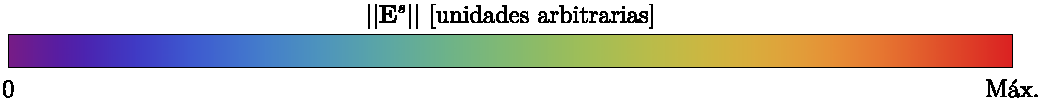
\includegraphics[scale=.85]{1-Teoria/figs/EsNorm.pdf}\\
%		\hspace{-4em}
%		\begin{subfigure}{.05\linewidth}\vspace{-3.25cm}\label{figs:ElectricMultipoles} \caption{ } \end{subfigure}
%		\hspace{-3em}
%		\begin{subfigure}{.9\linewidth}
%		\animategraphics[loop, autoplay,scale=.25]{10}{1-Teoria/figs/Ne11/Ne11_crop-}{0}{62}%
%		\animategraphics[loop, autoplay,scale=.25]{10}{1-Teoria/figs/Ne12/Ne12_crop-}{0}{62}%
%		\animategraphics[loop, autoplay,scale=.25]{10}{1-Teoria/figs/Ne13/Ne13_crop-}{0}{62}%
%		\animategraphics[loop, autoplay,scale=.25]{10}{1-Teoria/figs/Ne14/Ne14_crop-}{0}{62}
%		\end{subfigure}\\
%		\hspace{-4em}	
%		\begin{subfigure}{.05\linewidth}\vspace{-3.25cm}\label{figs:MagneticMultipoles} \caption{ } \end{subfigure}
%		\hspace{-3em}
%		\begin{subfigure}{.9\linewidth}			
%		\animategraphics[loop, autoplay,scale=.25]{10}{1-Teoria/figs/Mo11/Mo11_crop-}{0}{62}%
%		\animategraphics[loop, autoplay,scale=.25]{10}{1-Teoria/figs/Mo12/Mo12_crop-}{0}{62}%
%		\animategraphics[loop, autoplay,scale=.25]{10}{1-Teoria/figs/Mo13/Mo13_crop-}{0}{62}%
%		\animategraphics[loop, autoplay,scale=.25]{10}{1-Teoria/figs/Mo14/Mo14_crop-}{0}{62}%
%		\end{subfigure}
%		\caption{Contribuciones multipolares \textbf{a)} eléctricas $a_\ell$ y \textbf{b)} magnéticas $b_\ell$ de orden $\ell = 1,2,3$ y $4$ del campo esparcido $\vb{E}^s$ por una partícula esférica, evaluadas en una superficie matemática esférica y concéntrica a la partícula que radía los campos EMs, en donde el plano de la página corresponde al plano de oscilación del campo eléctrico incidente $\vb{E}^i$. En las gráficas presentadas, el color rojo corresponde a los valores máximos del campo eléctrico, mientras que los azules son los puntos menos intensos, donde se presentan los nodos en la superficie esférica.}
%		\label{fig:Multipolos}
%	\end{figure}
	\begin{figure}[h!]\centering
		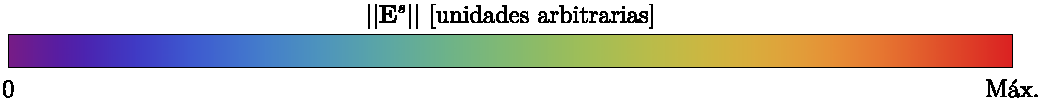
\includegraphics[scale=.85]{1-Teoria/figs/EsNorm.pdf}\\
		\hspace{-4em}
		\begin{subfigure}{.05\linewidth}\vspace{-3.25cm}\label{figs:ElectricMultipoles} \caption{ } \end{subfigure}
		\hspace{-3em}
		\begin{subfigure}{.9\linewidth}
			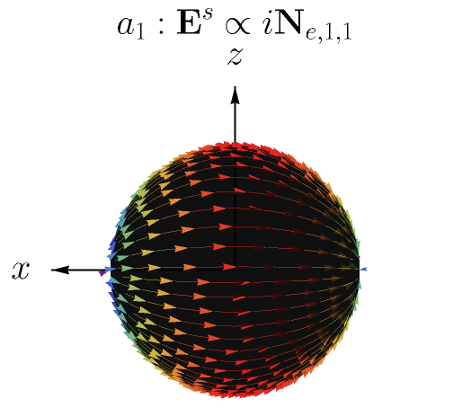
\includegraphics[scale=.25]{1-Teoria/figs/Ne11_static_crop.png}%
			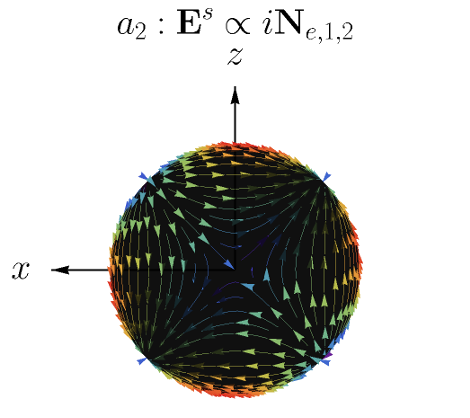
\includegraphics[scale=.25]{1-Teoria/figs/Ne12_static_crop.png}%
			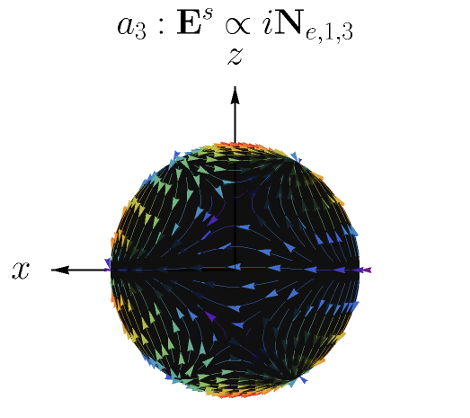
\includegraphics[scale=.25]{1-Teoria/figs/Ne13_static_crop.png}%
			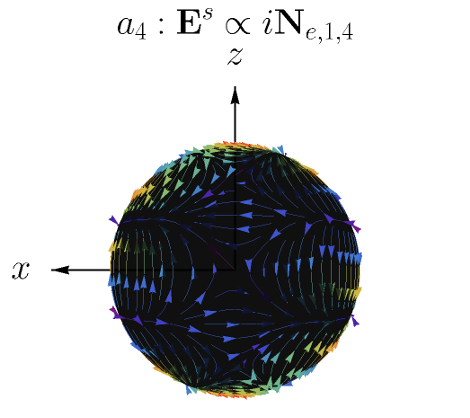
\includegraphics[scale=.25]{1-Teoria/figs/Ne14_static_crop.png}%
		\end{subfigure}\\
		\hspace{-4em}	
		\begin{subfigure}{.05\linewidth}\vspace{-3.25cm}\label{figs:MagneticMultipoles} \caption{ } \end{subfigure}
		\hspace{-3em}
		\begin{subfigure}{.9\linewidth}			
		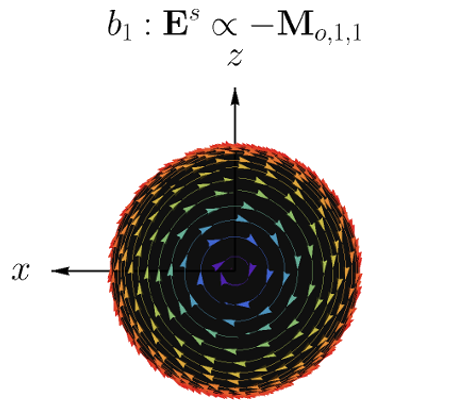
\includegraphics[scale=.25]{1-Teoria/figs/Mo11_static_crop.png}%
		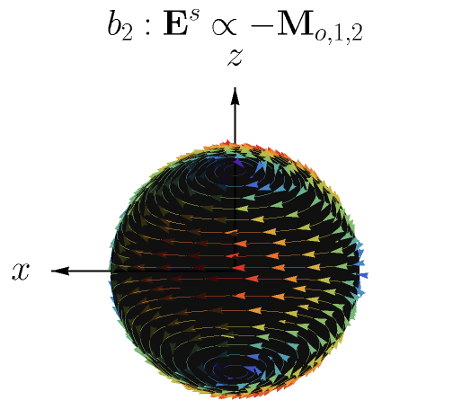
\includegraphics[scale=.25]{1-Teoria/figs/Mo12_static_crop.png}%
		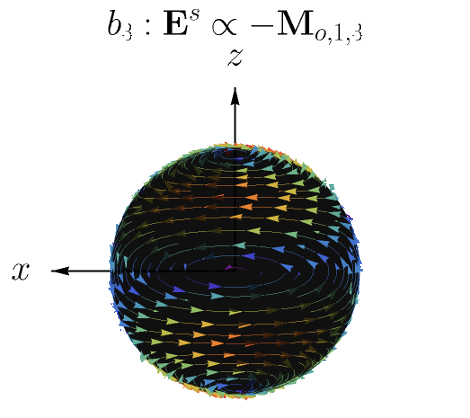
\includegraphics[scale=.25]{1-Teoria/figs/Mo13_static_crop.png}%
		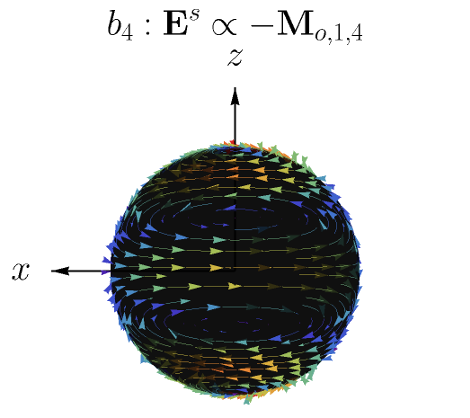
\includegraphics[scale=.25]{1-Teoria/figs/Mo14_static_crop.png}%
		\end{subfigure}
		\caption{Contribuciones multipolares \textbf{a)} eléctricas $a_\ell$ y \textbf{b)} magnéticas $b_\ell$ de orden $\ell = 1,2,3$ y $4$ del campo esparcido $\vb{E}^s$ por una partícula esférica, evaluadas en una superficie matemática esférica y concéntrica a la partícula que radia los campos EMs, en donde el plano de la página corresponde al plano de oscilación del campo eléctrico incidente $\vb{E}^i$. En las gráficas presentadas, el color rojo corresponde a los valores máximos del campo eléctrico, mientras que los azules son los puntos menos intensos, donde se presentan los nodos ($\vb{E}^s\approx \vb{0}$) en la superficie esférica.}
		\label{fig:Multipolos}
	\end{figure}

Los campos EMs esparcidos [Ecs. \eqref{eq:EHsAEV}] se calcularon al considerar una onda plana monocromática incidente $\vb{E}^i$ polarizada en la dirección $\vu{e}_x$. Sin embargo, debido a la simetría de la esfera, una onda plana polarizada en la dirección $\vu{e}_y$ se describe mediante la transformación $\varphi\to\varphi+\pi/2$, por lo que los campos EMs esparcidos y dentro de la esfera se calculan mediante el mismo procedimiento \cite{bohren1998absorption}. Entonces, cualquier cantidad relacionada con la absorción y esparcimiento de una esfera se puede calcular únicamente mediante lo coeficientes de Mie [Ecs. \eqref{eq:MieCoef}]. En particular, para determinar la matriz de esparcimiento $\mathbb{S}$ se relaciona el campo eléctrico esparcido en el límite de campo lejano\index{Electromagnéticos!campos!lejano}, en donde al emplear las funciones de Riccati-Bessel, y sus derivadas, en el límite asintótico\footnote{\index{Ricatti-Bessel!funciones de!límite asintótico de las}\index{Hankel!funciones esféricas de!límite asintótico de las}En el límite $\ell^2 \ll \rho$, se cumple que $h_\ell^{(1)}(\rho)\approx (-i)^\ell e^{i\rho}/i\rho$ y $\dv*{h_\ell^{(1)}}{\rho} = (-i)^\ell e^{i\rho}/\rho$. Por lo tanto,  $\xi(\rho)\approx (-i)^\ell e^{i\rho}/i$ y $\dv*{\xi}{\rho} = (-i)^\ell e^{i\rho}(1/i\rho + 1)$.} $\ell^2 \ll kr$, las componentes radiales de los campos EMs decaen como $(k_mr)^{-2}$, por lo que son despreciables. Al escribir los armónicos esféricos vectoriales [Ecs. \eqref{eq:AEV}] en términos de $\pi_\ell$, $\tau_\ell$ y de las funciones de Riccati--Bessel $\psi$ y $\xi$ en el límite asintótico, despreciando los términos proporcionales a $(k_mr)^{-1}$, el campo eléctrico esparcido en la componente paralela y perpendicular al plano de esparcimiento (ver Fig. \ref{fig:PlanoEsparcimiento}) es
	\begin{subequations}
	\begin{align}
	E_\theta^s \vu{e}_\parallel^s &=\frac{\cos\varphi}{k_mr}
								\sum_\ell^\infty E_0i^\ell\frac{2\ell+1}{\ell(\ell+1)}
						(i a_\ell\xi_\ell'\tau_\ell-b_\ell\xi_\ell\pi_\ell)\vu{e}_\theta\notag\\
			&\approx E_0\cos\varphi\frac{e^{ik_mr}}{-ik_mr}\sum_\ell^\infty\frac{2\ell+1}{\ell(\ell+1)}
				( a_\ell \tau_\ell + b_\ell\pi_\ell )\vu{e}_\theta ,
				\label{seq:EsFF}\\
		E_\varphi^s \vu{e}_\perp^s &= \frac{\sin\varphi}{k_mr}
							\sum_\ell^\infty E_0i^\ell\frac{2\ell+1}{\ell(\ell+1)}						
							(-ia_\ell\xi_\ell'\pi_\ell+b_\ell\xi_\ell\tau_\ell)\vu{e}_\varphi \notag\\
			&\approx E_0\sin\varphi\frac{e^{ik_mr}}{-ik_mr}\sum_\ell^\infty\frac{2\ell+1}{\ell(\ell+1)}
			(a_\ell\pi_\ell+b_\ell\tau_\ell)(-\vu{e}_\varphi), \label{seq:HsFF}
	\end{align}\label{eq:EHsFF}
	\end{subequations}
\! donde $\vu{e}_\parallel^s =\vu{e}_\theta$ y $\vu{e}_\perp^s=-\vu{e}_\varphi$. Al emplear la Ec. \eqref{eq:EIncidente} para reescribir a la onda plana incidente $\vb{E}^i$ [Ec. \eqref{eqs:EiAEV}] en la base de $\{\vu{e}_\parallel^i,\vu{e}_\perp^i\}$ [Ec. \eqref{eqs:vecInc}], se determina la forma explícita de la matriz de esparcimiento para una partícula esférica:\vspace*{-.75em} \index{Mie!matriz de esparcimiento de}\index{Esparcimiento!de Mie, matriz de}
	\begin{tcolorbox}[title = Matriz de esparcimiento de Mie,  breakable ]
	\begin{align}
	\mqty(E_{\parallel}^s\\E_{\perp}^s)  =  
		\frac{e^{ik_m(r-z)}}{-ik_mr} \mqty(S_2 (\theta) & 0\\ 0 & S_1 (\theta))
	\mqty(E_{\parallel}^i\\E_{\perp}^i),	
	\label{eq:MieMatrix}
	\end{align}
	donde $E^i_\parallel=E_0\cos\varphi$, $E^i_\perp = E_0\sin\varphi$ y \begin{subequations}\\
	\eqhalf{	S_1 (\theta) = \sum_\ell^\infty\frac{2\ell+1}{\ell(\ell+1)}(a_\ell\pi_\ell+b_\ell\tau_\ell),
				\label{eqs:S_1}}
	\eqhalf{	S_2 (\theta) = \sum_\ell^\infty\frac{2\ell+1}{\ell(\ell+1)}( a_\ell \tau_\ell + b_\ell\pi_\ell ).
			 \label{eqs:S_2}	}
	\label{eq:MatrixElements}	\end{subequations}
	\end{tcolorbox}\vspace*{-.75em}\noindent

